\chapter{INTRODUCTION}
\label{INTRODUCTION}
%Wireless networks utilize radio waves instead of wires to carry information, hence seamless coverage and mobility are achievable in wireless connections.
Wireless networks have experienced unprecedented growth in the past few decades and will going on evolving in the future.
Due to the propagation characteristics and regulations, only a small portion of electromagnetic spectrum which spans from 8.3 kHz to 3000 GHz is suitable for commercial application.
These spectrum is divided into bands (also referred as channels) and allocated to different services.
%In the following, we introduce how is the spectrum accessed by different services.
%
As one kind of limited and precious resource, radio spectrum is strictly regulated by the national administration.
The channels are assigned or leased by governments to different operators and entities.
In most cases, the operators pay high price for the commercial usage of certain spectrum, and the usage is exclusive for them~\cite{Spectrum_Management07}.
This spectrum management policy rules out the unlicensed users to use the spectrum, thus strictly protects the interest of the spectrum licensees.
This spectrum access module is referred \textit{exclusive use model}~\cite{zhao_survey_DSA_2007}, and is the mainstream of spectrum access worldwide, and many existing wireless applications work on the licensed spectrum.
For instance, the second-generation (2G) wireless cellular network \gls{gsm} (global system for mobile communications) in Europe works with GSM-900 band (from 890 MHz to 960 MHz) and GSM-1800 (1710 MHz to 1880 MHz), and the third-generation (3G) wireless cellular network works from 1.8 GHz to 2.4 GHz~\cite{wireless_communicatioins2001}.
The excludability of licensed spectrum can also be open to other user with conditions.
The spectrum licences either sell and trade the licensed spectrum, or dynamically use the spectrum within a certain region according to different traffic patterns~\cite{dsa_traffic_2000}.
Open spectrum access~\cite{osa_Noam_1995} is proposed in 1995 for full openness of entry, which allows access to spectrum through access fees which are determined by demand and supply.
It is claimed that open spectrum access brings in benefits, as for spectrum licensees, the fixed costs on securing the licensed spectrum can be converted into marginal costs, and for the market, the incentives for collusive pricing can be eliminated.
But as the \textit{openness} here is fully controlled by the licensees, this spectrum usage is still exclusive .

%
In contrary to exclusive use model, certain spectrum are assigned for open sharing for peer users, the representative example is the unlicensed industrial, scientific, and medical (\gls{ISM}) radio band, which supports versatile wireless applications and a prosperous industry, \ie WiFi.
Many spectrum sharing strategies are proposed to cope with the technical challenges~\cite{Ko_DistributedCA}.

\section{Hierarchical Spectrum Access}
\label{hierarchical}
The proliferation of wireless network constantly arises urgent demand on bandwidth and throughput since the first generation of telecommunication in 1980s, which accordingly encourages the efficient use and reuse of the electromagnetic spectrum.
The next generation of telecommunication technology \gls{5G}, which is reported to come true in 2020, requires a leap forward of spectrum efficiency~\cite{5G_2014}.
The resorted applications under the label of 5G~\cite{5directions5G_2014}, \ie machine to machine communication, internet of things, etc, requires high speed and lower investment cost, but this is changeling as the achieved capacity approaches Shannon capacity, and most spectrum are licensed.
Meanwhile, the actual spectrum usage measurement conducted by FCC tells that at many locations or time, the licensed spectrum is idle~\cite{FCC_spectrumEfficiency_2002}, and there exists a large number of spectrum bands which have considerable dormant time intervals ~\cite{Akyildiz06survey}.


To seek more opportunities from spectrum, it is natural to consider opening the licensed spectrum to unlicensed users, if the interference perceived by licensed users are restricted.
We adopt the terms proposed in~\cite{zhao_survey_DSA_2007}, and call this spectrum usage policy as \textit{hierarchical access model}, where licensed users are called primary users (\glspl{PU}), and unlicensed users are named as secondary users.
Hierarchical access model gives a promising solution to the reclamation of new electromagnetic spectrum and the improvement of spectrum efficiency.




%\subsection{Spectrum Access Etiquette in Cognitive Radio Network}
%
%%CR users utilize the unused licensed spectrum opportunistically and meanwhile avoid interfering licensed users.
%%This new spectrum usage paradigm imposes great challenge to the CR users, including how to detect the licensed users and afterwards decide on the suitable spectrum and on which interact with other CR users.
%
%%Before the emerging of cognitive radio technology, spectrum is allocated in a fixed way, \ie certain chunk of spectrum is exclusively licensed to an certain entity by administration body.
%%The equipments which are given the license to utilize the spectrum is called licensed users, while the others which called unlicensed users are not allowed to work on the that part of spectrum.
%%This paradigm rigidly protects the benefit of licensed users, but it results in underutilization of spectrum.
%%Due to the drastic increase of mobile data applications there is an urgent demand on spectrum resources. 
%%Traditionally, frequency bands have been assigned exclusively to licensed bodies which can occupy the spectrum whenever there is information to be transmitted. 
%
%%This static spectrum utilization has been proven to be suitable for many systems and applications. 
%%However, as mobile networks have proliferated drastically over the last thirty years, this exclusive assignment has created a significant shortage of spectrum today. 
%
%Licensed users access their allocated spectrum band whenever there is information to be transmitted, in contrary, CR users are only allowed to access licensed spectrum after validating the channel is idle or the primary user is not to be affected if they operate on the licensed spectrum.
%In this thesis, licensed users are referred as primary users, and CR users are denoted as secondary users.
%
%The assessment of spectrum is a bone of contention for primary/secondary users and administration bodies.
%Spectrum sensing on secondary users is one common method to validate spectrum availability especially in research domain~\cite{crnsensing_09}.
%%Secondary users should monitor the spectrum of interest actively and autonomously to detect primary users' appearance.
%%Primary users can be detected by judging the primary users' signal power, spectral correlation or beacons.
%%Spectrum sensing requires sophisticated technologies when primary users' signal is weak.
%%Primary detection can be improved by learning technologies or cooperation among multiple secondary users~\cite{coorperativeSensing_Akyildiz11}.
%Another way to protect the primary users from being affected by secondary users' operation relies on location identification and certain operating rule set.
%Based on the global information of primary users' location and terrain information, centralized controller regulates that the secondary users at certain locations are restricted to operate on a few certain spectrum bands and with limited transmit power~\cite{whitefi09}.



%In contrast, CR users (forming cognitive radio networks, abbreviated as CRN) 
%This refers to the process of sensing a particular channel and verifying (with a previously specified probability of error) that it is not used by a primary user currently  [cite spectrum sensing].
%This form of spectrum sharing is also referred to as opportunistic spectrum access~\cite{Akyildiz06survey}.

%Such co-existence with primary users imposes great challenges for the CR users.
%On the first hand, CR users should be able to sense the channel to avoid interfering primary users.
%it is fairly easy to see that the sensing ability of secondary users plays an important role in the harmonious co-existence of primary and secondary users~\cite{09spectrumSensing_survey}.





\section{Cognitive Radio}
%\cite{spectrumSharingGames_interference_stackelberg_2009, spectrum_sharing_games_2010} spacial opportunistic allocation.


Throughout this thesis, we use \textit{cognitive radio networks} to compound the networks composed with secondary users which work in either spectrum underlay or spectrum overlay style.
There are two reasons, firstly, this name explicitly tells a distinctive property of the devices in the networks, their cognition to their environment, secondly, cognitive radio has become a synonym of the technology employed in the hierarchical spectrum access paradigm in academia and industry in the recent years.



%The dilemma that spectrum scarcity coexists with spectrum underutilization promotes cognitive radio (CR) as a promising technology to make full use of spectrum and accordingly solve the spectrum shortage problem.

The definition of cognitive radio evolves with the development of radio technology and regulations.
We choose two representative definitions to give a formal description of cognitive radio.
Cognitive radio (\gls{CR}) is firstly proposed by Mitola III who defines the concept of CR in his dissertation~\cite{2000mitola_cognitive_radio} as follows:
%
\blockquote{... personal digital assistants (\glspl{PDA}) and the related networks are sufficiently computationally intelligent about radio resources and related computer-to-computer communications to detect user communications needs as a function of use context, and to provide radio resources and wireless services most appropriate to those needs.
}

FCC (Federal Communications Commission in U.S.) describes CR~\cite{FCC_03-322} as,
\blockquote{
a radio that can change its transmitter parameters based on interaction with the environment in which it operates. $\ldots$
This interaction may involve active negotiations with other spectrum users and/or passive sensing and decision making (smart radio) within the radio. The majority of CRs will probably be SDRs~\footnote{software defined radio is a radio communication system which is able to receive any modulation across a large frequency spectrum, and transmit on desired spectrum band.}, but a CR does not necessarily use software, nor does it need to be field programmable.
}

In this thesis, we see cognitive radio as a device which is able to sense, detect, learn and monitor the surrounding radio frequency environment, or to access a certain database to retrieve primary users' information, so as to reconfigure its radio operating parameters (\eg center frequency, bandwidth and transmit power) on the fly to avoid interfering primary users.
Cognitive radio may only practice one portion of the aforementioned functionalities according to actual situation.
Apparently, the cognitive radio users which conduct spectrum sensing are usually work with spectrum overlay paradigm, and the cognitive radio users which have means to get information of primary users are suitable to work with spectrum underlay paradigm.
Based on this definition, throughout this thesis the secondary users working with both spectrum underlay and overlay are named as cognitive radio users, besides, the cognitive radio network is deemed to be composed with cognitive radio users, whose acronym is \gls{CRN}.



\subsection{Spectrum Management}
To adapt to dynamic spectrum environment and make use of the available licensed spectrum, cognitive radio users need to manage the available spectrum by conducting the following procedures sequentially, detecting the available spectrum with spectrum sensing, selecting the proper spectrum for communication, and sharing the spectrum with other secondary users.
These functions are incorporated into so called cognitive cycle as described in~\cite{Akyildiz09}.

\subsubsection*{Spectrum Sensing}
To know which chunk of spectrum is available is the foundation of spectrum management.
In underlay spectrum usage scenario, CR users get to know the available spectrum by means of spectrum sensing.
In overlay spectrum usage scenario, secondary users can in principle access all the licensed spectrum.
In this procedure, quality of the available channels is determined with several parameters, \ie band width, operating frequency, path loss, wireless link errors, link layer delay, and the upper bound of interference on the primary user working on that channel, which decides the maximal permissible transmission power of secondary users.
Besides, the statistical behaviours of primary users is also an important factor.

\subsubsection*{Spectrum Decision}
After knowing the available spectrum, CR users select the most appropriate band according to their requirements on quality of service (QoS).
This procedure involves considering the statistical behaviours of the primary users so as to accessing the channel quality fairly.
%


\subsubsection*{Spectrum Sharing}
Then secondary users are to make use of these selected channels, or in other words, to share the spectrum with other secondary users. 
As there may be multiple secondary users trying to use the same channel, spectrum sharing is important to coordinate the behaviour of secondary users to avoid deteriorating the performance of secondary users.
Spectrum sharing involves choosing proper channels to mitigate co-channel or adjacent interference, or adjusting transmission power to achieve promise between transmitter's and other secondary users' performance, or adopting a certain media access paradigm to use the spectrum fairly and efficiently.
Spectrum sharing also involves consideration on primary users, \ie when many secondary users work on the same channel, the accumulated interference caused by secondary users could exceed the interference threshold on primary users.
%\todo[inline]{spectrum opportunity, detection, tracking, exploitation (whether to access, how to access, sharing),  tazhaosurveyDSA2007.}

%According to \cite{08crn_survey}, 	
%After assessing RF environment or geographic location, secondary users adjust their operational parameters such as frequency, modulation schemes and transmit power, in order to support QoS aware communications, this process is referred as spectrum decision and spectrum sharing~\cite{08crn_survey}.
%In this thesis, spectrum decision and sharing consist the major issue discussed in this thesis.

Some work in research community models the spectrum availability with stochastic or statistic model, which is helpful when deciding which channel to use.
\cite{Discrete-Time_Spectrum_Occupancy_Model_DySPAN_2011} proposes discrete Markov chain and adjusts duty circle models to describe the availability of licensed spectrum for GSM on 900/1800 MHz.
\cite{Wellens200910} models the channel holding time with geometric and log-normal distributions.
Statistics of previous sensing results is used to predict spectrum state in the future~\cite{spectrum-discovery-tmc08}.
Such models provide more complete information on the availability of the licensed channels.

The available licensed spectrum which spans a wide frequency band exhibits different characteristics~\cite{spectrum_decision_TMC11}.
Based on the requirements of interested communication, CR users need to identify the characteristics of the spectrum, which include channel quality (channel capacity, error rate, path loss, etc.)~\cite{spectrum_decision_TMC11}, channel switching delay~\cite{channel_switch_delay11}, and channel holding time, \ie the expected time duration that the primary users don't occupy the channel before any one occupies again.



\subsection{Representative Cognitive Radio Networks}
In this section, we introduce two types of cognitive radio networks, and the problems we tackle in this thesis reside in these networks.

\subsubsection*{Cognitive Radio Ad Hoc Network}
%An ad hoc network is a decentralized paradigm of wireless network, which consists of a collection of autonomous mobile users which communicate over wireless links.

%Efficient distributed algorithms are needed to determine network organization, link scheduling, and routing.

Cognitive radio ad hoc network (\gls{CRAHN}) is composed with autonomous mobile cognitive radio users which work with overlay spectrum sharing paradigm.
CRAHN is usually represented as an undirected graph $G$.
Cognitive radio users constitute the vertices, the edge between two vertices is decided not only by the distance, propagation and attenuation properties between the two vertices, but also the spectrum availability on both vertices, \ie when they can decode the received signal from each other correctly, and there is common channel available between them on which communication is conducted, then an bidirectional edge is available on graph $G$.
As to ad hoc network, the graph is constant when users are static.
As to cognitive radio ad hoc network, due to primary users' activity, an edge between two vertices is decided by the fact that whether the two vertices can simultaneously access the same licensed channel.
Hence, the corresponding graph is dynamic under primary users' operation, which imposes extra difficulties on network organization, routing and many other network functionalities.

\subsubsection*{IEEE 802.22 Standards}
\label{ieee80222}%XXXXXXXXXXXXXX clearly statement, regulations of FCC, ECC, 802.22 XXXXXXXXXXXXXXXXXXXX
%%XXXXXXXXXXXXXXXXXXXXXXXXXXXX   paper: IEEE 802.22: The First Cognitive Radio Wireless Regional Area Networks (WRANs) Standard
IEEE 802.22~\cite{802.22} is the standard for Wireless Regional Area Networks (\glspl{WRAN}), which defines a cellular network paradigm for secondary equipments working on unused TV channels in overlay manner.
Unused TV spectrum is termed as TV White space by the Federal Communications Commission (FCC)~\cite{FCC_2010_sedond_memorandumm}, which is licensed to incumbent users such like digital TV, analog TV, and wireless microphone.
As the TV service is transferred from traditional analog to digital, the
The TV channels to be used are of UHF/VHF TV bands and are between 54 and 862 MHz.
The bandwidth of one TV channel is 6 MHz.%XXXXXXXXXXXXX add some description in details XXXXXXXXXXXXXXXXXXXXXX


Unlicensed users consists of White Base Stations (\glspl{WBS}) and customer premises equipments (or terminals for short), where each terminal is served by one base station. 
As to unlicensed users, detecting incumbent users is challenging because the FCC requires the unlicensed users should be able to detect the presence of signals from TV stations or wireless microphone at a received power level of -114 dBm~\cite{Technical_Challenges_TVwhit}. 
Thus FCC doesn't require the sensing ability on unlicensed users, but regulates the secondary usage of TV white space in a prudent manner, including the spectrum bands permitted to use based on their location, the transmission power, the distance away from TV service area and so on.
IEEE 802.22 largely complies FCC regulations on the utilization of TVWS.

There exists a centralized database, and every unlicensed user should register its type and geographic location to one TV database.
The centralized database notifies the secondary users the available spectrum at their places, and is possible to decide transmission parameters for them, \ie spectrum to be used, or transmission power.
Note this database takes the functionality of spectrum sensing in addition to spectrum decision and sharing, thus IEEE 802.22 adopts centralized spectrum decision for unlicensed users.
The feasibility of this centralised paradigm is largely due to the characteristics of TV channel, as TV channel usage follows a slow and scheduled pattern. 
When two or more base stations operate on the same channel, TDMA like mechanism for WBSes is adopted.
%Centralized spectrum decision is adopted in IEEE 802.22.





Recent standard published in Nov. 2010 suggests both sensing ability as well as database look-up to avoid affecting primary systems.
%As to utilization of available TVWS, IEEE 802.22 proposes centralized channel allocation in database.



\subsubsection*{TV White Space}
%Opportunistic utilization for unlicensed secondary users (also named as white space devices, abbreviated as WSD) working with TV broadcast spectrum (TV white space) is promising to cope with the scarcity of spectrum resources\cite{fcc}. 
%UHF TV spectrum (TV white space, TVWS) has low utilization in both spatial and temporal dimensions. \fmjg{xxx relevant data and citation needed here XX also mention where this is the case, i.e. US ? XXX} 

Locating in the VHF and UHF bands, TV White Spaces (TV white space, TVWS) are highly desirable for wireless communications, because they have good properties on propagation, buildings penetration, and broadband payload capacity. In the US, the requirements for secondary spectrum usage in the TV broadcast bands are given by FCC. 
%
On November 4, 2008, FCC made far reaching changes by opening the unused portion of the UHF TV space to unlicensed secondary users. \textit{Unused portion} here denotes the TV spectrum which is not currently being used by TV stations, or that secondary users can use while the ongoing TV broadcasting on the same spectrum is not interfered.
%
As mentioned, autonomous spectrum sensing is one approach for secondary users to decide the available TV spectrum. With sensing ability, every secondary user scans certain parts of the TV spectrum band and is able to detect TV transmission even from a very distant place such that those channels\footnote{In the following, we use the words \textit{spectrum} and \textit{channel} interchangeably.} can be ruled out for usage. However, to real prevent any interference with ongoing TV broadcasts, the sensing algorithm becomes quite complex. Moreover, it is required to be conservative when deciding the available TV channels leading to an underestimation of available TV channels and causing inefficiencies~\cite{geoTVprotection08dyspan}. Considering the slow change of TV spectrum usage, along with the fact that the spectrum usage by TV stations is scheduled, the geolocation approach together with central database becomes more appealing in TVWS (TW White Space) utilization scenario. FCC adopts this solution as the main way, and regulates the secondary usage of TV white space in a prudent manner, including the spectrum bands permitted to use based on their location, the transmission power, the distance away from TV service area and so on. FCC regulates portable secondary users to operate from channel 21 (512 MHz) to 51 (698 MHz), with the exception of channel 37. As to fixed secondary usage, the allowed spectrum band is from TV channel 2 (54 MHz) to TV channel 51, with TV channels 3, 4 and 37 being prohibited. Thus, the available TV spectrum is about 600 MHz wide. Compared to conventional unlicensed ISM bands in the 2.4 GHz and 5 GHz band, all together TVWS has more to offer.

While the TV spectrum is free to use under the above mentioned conditions, it might also be 'polluted' by primary TV stations due to the coexistence with them. \cite{DySpAN10MeasuringWhitespaceCapacity} analyzes the capacity possibly provided by exploiting free TV channels. Complying with the rigid regulation of FCC, TV white space brings hundreds of kilobits/sec per square kilometer for secondary users when the communicating secondary pair is about 1 km apart. The research shows that interference from TV stations and other co-channel secondary users heavily restricts the capacity. \cite{tvgreyspace12} further investigates the possible TVWS usage \textit{within} TV service area (referred to as 'gray space'), where the secondary usage does not violate TV receivers. The authors propose another significant amount of TV spectrum, but the interference from TV broadcasters is stronger due to the secondary receivers being closer to TV broadcasters. 

The potential applications supported by TVWS are the major driving force for TVWS communications technology. It is envisioned that TVWS can support high-data-rate backbone for fixed stations in Large Area Connectivity, short-range indoor connectivity, seamless connectivity for mobile stations and emergency related equipment. In the following, we give a brief introduction to the governing regulations and industrial standards issued for TVWS usage.
%



%Firstly, more unused TV white frequencies become vacant than ever with the ongoing transition from analog to digital broadcasts. Secondly, the lower frequencies of TV band enable broadband access over much longer ranges compared to other bands with higher center frequencies. TV white space contributes an alternative to industrial, scientific, and medical (ISM) band which is already heavily congested. Besides, TV white space provides abundant spectrum resources for cellular network, so that the frequency reuse factor is decreased and sophisticated interference mitigation mechanisms can be alleviated. TVWS is free but with restrictions, TV receivers should be protected from the harmful interferences form WBDs, in other word, the aggregated interferences caused by all working WSDs should not exceed a threshold on TV receivers.



\subsubsection*{Co-Existence in TV White Space}
%In compliance with the methodology of cognitive radio, 

%this is a intro to a general cr work.
%Temperature regulation~\cite{Temperature_regulation03} opens another way to utilize TVWS. \cite{wuinfocom09} deals with the joint channel-power selection for multiple transmission links (pairs) in a general cognitive radio scenario. The distributed scheme is derived from decomposition of Lagrangian dual, which converges pure Nash equilibrium. To facilitate this scheme, monitors from TV stations are required to watch interference from WSDs, furthermore, monitors have to be equipped with computational ability and interact with secondary users in the whole process of convergence. This methodology works in try-error-try mode, which asks for modification on the current operation of TV services.
Regulatory bodies in different countries have issued requirements on the occupancy of TVWS bands, respectively. The permissible channels regulated by FCC have been briefly introduced above. Besides, FCC divides the devices operating in the TVWS (TV band devices, or TVBDs) into three categories: Fixed device, Mode I personal/portable device, and Mode II personal/portable device. Every category obeys different rules on transmission power, mandatory database access and so on. Fixed and Mode II devices are connected to the database directly (or indirectly by another fixed or Mode II TVBD), Fixed device accesses DB at least once per day, Mode II device has to access DB every 60 seconds, or when it changes location by more than 100 meters. The transmission power for Fixed TVBD is 4 W, and 100 mW for Mode II TVBD. Mode I TVBD operates only under the control of a fixed or Mode II TVBD, and accesses them for available channels every 60 seconds. There is also regulations on the antenna heights and other aspects. OFCOM (being the regulatory authority in UK) opens less TVWS for TVBD and categorizes White Space Devices (WSDs) into Master WSD and Slave WSD which are roughly equivalent to fixed/Mode II TVBD and Mode I TVBD, respectively. ECC (being the regulatory authority in Europe) also adopts Master and Slave structure while utilizing the geolocation and database solution to assign channels and corresponding operating parameters to TVBD. In both FCC and ECC regulations, the available channels are calculated based on the distance between primary and secondary systems together with some propagation model. Hence, the principle behind the notion of channel availability is the presumed received signal strength at potential TV receivers, which should be obviously below a certain level. FCC adopts a fixed transmit power level for secondary systems and assumes that the distance used (resulting from the propagation model) is sufficient to protect the TV receivers. ECC's restriction is more flexible on the transmission power which can be adjusted based on the distance between the secondary user and the TV receivers. For both regulations, TV receivers may become vulnerable when there are multiple secondary equipments transmitting simultaneously. \cite{Jaentti11} shows that even the regulations integrate an interference margin for multiple secondary users' transmitting, the TV receivers are still vulnerable.

%
%Some regulations, as that from FCC and ECC, are sufficient guidance for actual implementation, while some other rules are providing test for interference assessment. 
%
Standardization on secondary usage of TVWS is very active. IEEE 802.19 is a family of IEEE 802 standards in Wireless Coexistence Working Group, among which, IEEE 802.19.1 is for wireless coexistence in TVWS. IEEE 802.11af is standards for WLAN operation in TVWS, IEEE 802.15.4m is for low rate (LR) WPAN operating in TVWS. IEEE 802.22 is for Wireless Regional Area Network (WRAN) using TVWS. As TV band is only 6 or 7 MHz while WLAN channel bandwidth is 40 MHz for state-of-the-art IEEE 802.11n amendment, IEEE 802.11af proposes channel aggregation mechanism for WLAN working with TVWS. Maximum transmit power and spectrum mask of Mode I should be approved by Mode II devices beforehand.  


%Geolocation is extensively used in cognitive radio network. \cite{nashbargaining_2012jsac} proposes a centralized light weighted scheme to solve channel and power allocation among secondary users with TDMA manner, where geolocation of primary users are used by secondary users to calculate the caused interferences by them on the primary users. Considering the slow change of TV spectrum usage, along with the fact that the TV spectrum usage is scheduled, geolocation approach becomes more appealing in TVWS utilization scenario. Assume there is a database which is connected with all WSDs, and it is aware of the location of TV receivers (optionally with terrain information) and WSDs and proper propagation model in between, the database calculates the RSSI (Received Signal Strength indication) on each WSDs in the whole network. The database decides the channel availability based on whether the RSSI exceeds a threshold value or not, then notices WSDs their available channels in either proactive or reactive manner. This geolocation approach is used for building a WiFi like network working with TVWS ~\cite{SenseLess} which demonstrates the feasibility of predicting the available TV spectrum accurately using suitable propagation models (Longley-Rice and terrain wherein). This approach is also integrated into regulation from Federal Communications Commission (FCC) of U.S. FCC regulates every WSD should access the database to retrieve the available TV channels on its location, and fixes the transmission power for fixed WSD as 4 W which is a conservative value. Aforementioned is calculation RSSI of PU on the location of WSDs to see whether the PUs \textit{appears}, there is another way to work with geolocation. Instead of deciding the available TV channels for WSDs, database calculates the interferences from WSBs on TV receivers, then directly assigns channel and power levels to each WSD and in the same time preventing the TV receivers from harmful interferences (the interferences under a certain threshold). Electronic Communications Committee (ECC) in Europe adopts this approach so that the transmission power for WSD is more flexible depending on WSD's location.


IEEE 802.22 has been the first IEEE standard for wireless regional area network (WRAN) working on TV white space. According to this standard, the system consists of a base station and customer premises equipment (or terminals for short), where terminals are associated with base stations, and are served by them. Recent standard published in Nov. 2010 mentions both, i.e. sensing ability as well as TVWS geolocation and database look-up as schemes for detecting primary systems. Self-coexistence mechanism is also proposed, which provides a TDMA like mechanism for WBSes to share TVWS. \cite{HoangPowerChannel2010} proposes a distributed solution for power control and channel assignment in both down-link and up-link communication in a WRAN, but the investigated secondary network is composed with only one base station and multiple terminals. % Although the transmission power is decided in a distributed manner, primary transmitters are required to adjust their transmission power in order to guarantee the SINR on primary receivers in a learning process, while, the operation of WSDs working on TVWS should be transparent as to TV services.\fmjg{This summary of the 2010 paper does not make sense to me - why are you talking of primary systems here ??} 

Each base station working with TVWS needs a certain transmission power and a certain spectrum. The decision should maximize performance in this cell under interferences from TV broadcasters and other secondary base stations, meanwhile, the TV receivers should be protected. Up to our knowledge, there is no work coping with co-existence between secondary base station with both primary TV broadcasters and other base stations. %Considering that secondary base stations are likely to be from different administrative domains, a distributed solution would be required. And that makes us turn to game theory and the separation of the problem into two different ones. 
In the following, we propose a workaround for the joint power and channel allocation problem for WRAN composed with multiple base stations.





\section{Spectrum Sharing Paradigms}
How is the available licensed spectrum shared among secondary users is a fundamental problem in CRN, because it decides secondary users' performance, and it also poses threat to interferer primary users.
In this section, we introduce spectrum sharing from three different perspectives.

\subsection{Classification in Respect of the Relation between Primary and Secondary Users}
 sharing can also be classified by network architecture and spectrum allocation behaviour~\cite{Akyildiz09} respectively.
In this section, we introduce these classifications to vision spectrum sharing from different prospectives.

\subsubsection*{Spectrum Underlay}
One approach is \textit{spectrum underlay}, where the interference generated by secondary users on the primary receivers should be under a threshold. 
This kind of spectrum sharing restricts the secondary users' transmission power, but is able to achieve high data rate in short range.
When implementing spectrum underlay, secondary users are allowed to operate near the primary users when the interference caused on primary users is taken care~\cite{Ellingsaeter2012_Increasing_Available}.
Figure~\ref{underlay} shows a spectrum underlay sharing scenario, where some secondary users operate within the TV service area when the caused interference by the secondary users on the TV receiver is lower than threshold.

Spectrum underlay is mainly conducted with a centralized controller, which has global knowledge of primary users' location, the attenuation between all secondary transmitters and all primary receivers.
Then the centralized controller calculates the maximal permitted transmission power with certain optimization solutions in a situation where secondary users pose the maximal thread to primary users' operation, where all the secondary users work one the same licensed spectrum.
%secondary users at certain locations are restricted to operate on a few certain spectrum bands and with limited transmit power~\cite{whitefi09}.
%Given the attenuation between all secondary transmitters and all primary receivers and their locations, when the interference threshold is known, the maximal permitted transmission power levels of secondary transmitters can be obtained with linear programming.
Working with spectrum underlay paradigm, spectrum sensing functionality on secondary users becomes auxiliary~\cite{FCC_2010_sedond_memorandumm, ecc159}.
\begin{figure}[h!]
  \centering
  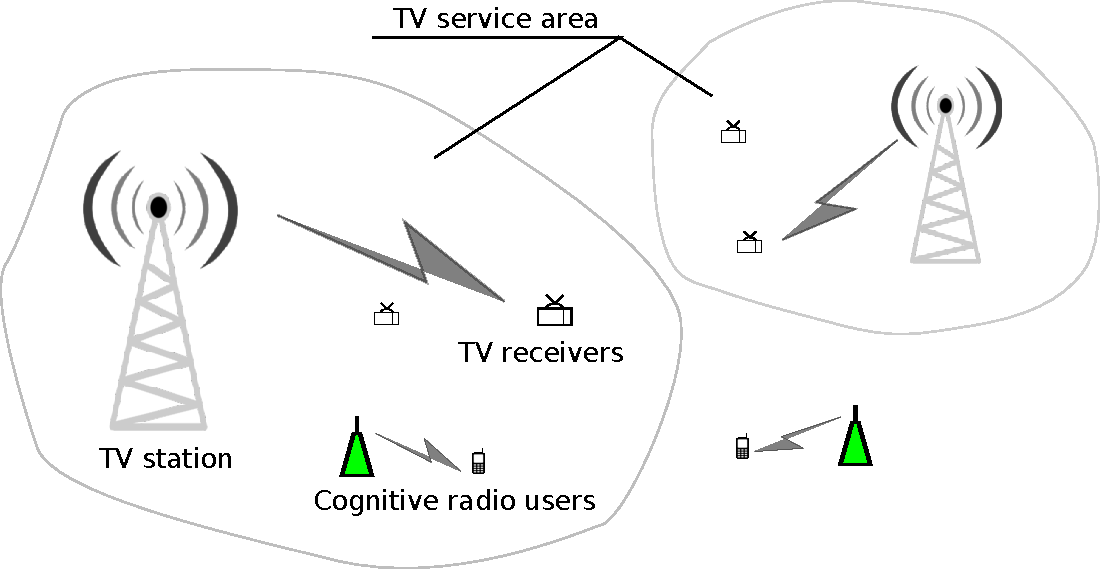
\includegraphics[width=0.75\linewidth]{underlay.pdf}
  \caption{The concept of overlay spectrum usage in a TV service scenario. The hull shows the range of a TV service area, inside and out of which secondary users work on the licensed channels.}
\label{underlay}
\end{figure}


\subsubsection*{Spectrum Overlay}
The other approach is \textit{spectrum overlay}, where secondary transmitters are only allowed to transmit when the primary users are detected as being idle.
In this paradigm, secondary users should monitor the spectrum of interest preactively to detect primary users' appearance.
The detection metrics include received primary users' signal power, spectral correlation or beacons~\cite{crnsensing_09}.
Spectrum sensing requires sophisticated technologies when primary users' signal is weak, and can be improved by learning technologies or cooperation among multiple secondary users~\cite{coorperativeSensing_Akyildiz11}.
When spectrum sensing accuracy can be guaranteed above certain threshold, transmission power restrictions can be removed from  secondary users.


%


Spectrum administration bodies FCC of U.S.~\cite{FCC_2010_sedond_memorandumm} and Electronic Communications Committee (\gls{ECC}) in Europe~\cite{ecc159} encourage to adopt both spectrum sensing and location based method.
%Secondary users' operation is restricted on certain spectrum bands and transmit power should be below certain threshold according  to their locations, and spectrum sensing ability is also required.



\subsection{Classification Based on Architecture}
Based on architecture, spectrum sharing can be classified as centralized and distributed spectrum sharing.

%Centralized spectrum decision doesn't work well outside the TV channel scenario.

\subsubsection*{Centralized Scheme}
Centralized spectrum sharing relies on a centralized entity where the strategy of spectrum usage is decided. 
There is considerable number of centralized approaches proposed for spectrum sharing in cognitive radio network, global optimality is reported as to different objectives, but centralized solution is not suitable in many real world situations.

First, central authority or controller is not available in many CRNs, \eg CRAHN.
Second, when the centralized decision maker exists, the centralized entity needs to collect spectrum availability sensed on all the secondary users, computes the spectrum usage strategy and distributes it.
A large number of control messages are generated during these processes.
When primary users intensely access the spectrum, resulting in frequent change of available spectrum, the control overhead becomes higher, and it is different for the centralized entity to obtain a full and up to date picture of the spectrum availability in the whole network .

Centralized scheme is suitable in certain scenarios, \eg when the primary users are TV stations and receivers which work on certain channels for hours of time, spectrum can be seen as constant. 
When the secondary users access the spectrum in underlay paradigm, they need to take care not to cause more interference than threshold on primary users.
In this case the channel usage, \ie working channel and transmission power, can be decided on the centralized controller.

%In wireless networks, signalling is performed to conduct resource allocation in an optimal way, which causes considerable overhead in communication.









%As to cognitive radio network, implementation of centralized algorithm faces more challenges.
%The central controller needs to know the network connectivity which is decided by the availability of licensed spectrum, or even the information of the later.
%Either the controller enquiring each secondary user for spectrum availability information, or the secondary users pushing to the controller introduces huge amount of overheads, especially when the primary users change their operation state frequently
%When the licensed users change their operation state frequently, centralized decision maker obtaining the updated sensing results from CR users imposes a great burden on the network.
%In this case, it is also possible that the centralized controller is only responsible to regulating the maximal transmission power to protect the licensed users from interference, but doesn't control secondary users' transmission strategy as they may belong to different business groups.

%Without infrastructure support, it is hard for CR user to get complete and up to date picture of the spectrum availability in the whole network.
%Thus distributed solutions are preferred in such varying radio environment.
%Distributed decision of one CR user should be carefully decided as one CR's behaviour affects neighbouring CR users which go on to prompt all the CR users in the network to act accordingly.

\subsubsection*{Decentralized Scheme}
Working with distributed spectrum sharing paradigm, secondary users autonomously decide their spectrum usage strategies.
Distributed scheme requires secondary users to exchange information \ie user ID, channel availability, etc. 
with its neighbourhood.
It is reported that control overhead takes more than 50\% of messages~\cite{Han:2008:RAW:1457343}.
If we can reduce the overhead, spectrum utilization and the number of users can be increased, and network performance can be improved.
Decision is made only with local information, as a result, communication overhead is reduced when the distributed decision has quick convergence. 
As distributed schemes exploit mainly local observation, distributed schemes adapt to the varying environment quite well~\cite{Selforganization_CRN_13}.

Distributed scheme may also make use of centralized entity when it is available and necessary, \ie secondary users can access the centralized database to retrieve available channels in IEEE 802.22 cellular networks.

%Signalling overhead is even more considerable as the channel state varies due to primary user activity.
%Thus the distributed scheme is more suitable than cognitive radio networks than other wireless networks.
It is challenging to design distributed schemes.
When the distributed decision is not properly designed, it is possible to trigger endless ripple effect across the network, \ie one CR's decision on its strategy prompts neighbouring CR users to change strategies, and it changes its strategy again later due to neighbours' new strategies.
In this thesis, the interaction between CR users will be discussed under game theoretical framework.
With certain utility function, secondary users' interaction is \textit{replicated} by a game which permits convergence.
As to some problems, we need to carefully design the utility function so as to make the corresponding game to converge.





%because it is costly to retrieve necessary information from the network to the controller, which includes the spectrum information on each CR users and the network topology. Besides, when the solution is sent back to the CR users, the network state may have changed and be different from the time when the information is collected.

%This is due to the operation of primary users, which is usually not known by secondary users.
%The distinctive view on spectrum availability and varying radio environment make distributed solution a natural choice for CRN network.





\subsection{Classification Based on Cooperate or Not}
Spectrum sharing can also be categorized into cooperative and non-cooperative spectrum sharing.
As to cooperative spectrum sharing, secondary users take into consideration of the caused interference on other secondary users when deciding their spectrum usage.
This pattern usually requires cluster structure to facilitate the negotiation of users in a neighbourhood~\cite{Chen07}.
Whereas with non-cooperative spectrum sharing, secondary users only consider the performance of their own.

Aforementioned classifications correlate with each other in certain aspects.
For instance, non-cooperative spectrum sharing is usually conducted in distributed manner, whereas cooperative spectrum sharing can be implemented in both distributed and centralized manner, and the later needs the assistance from the centralized entity.

%Spectrum sharing scheme need to be designed according to actual requirement and available facilities.








%The forthcoming vehicular to vehicular communication requires

%Based on the type of primary system which CRN underlays to co-exist, the availability of licensed spectrum exhibits variations on temporal and spatial aspects.



%However, the autonomous operation of secondary users always comes with a residual risk that primary systems are not detected despite their reappearance. Hence, other approaches to primary detection have been proposed relying on geolocation and database (DB), where secondary users are told by a centralized database about the spectrum availability with a time dimension. In this concept, the transmission power can also be controlled by the database. After obtaining the available spectrum to use, the secondary users need to decide which chunk of spectrum to use so as to satisfy the QoS requirements for the service it conveys. In order to achieve good performance, secondary users should be aware of the activity pattern of PUs, so that they can pro-actively plan the spectrum usage. Finally, SUs need to share the spectrum with other SUs, thus interference mitigation is an important issue to be considered.

%Whenever primary users are detected, the secondary users have to either jump to other spectrum, or turn down its transmission power to avoid interfering the primary users.





\section{Problem Statement}

In this thesis, the fundamental technical challenges to be addressed in this thesis are shown in Figure~\ref{problemLocation}, which reside from physical layer to network work layer~\cite{osi} are addressed. 


\begin{figure}[h!]
  \centering
  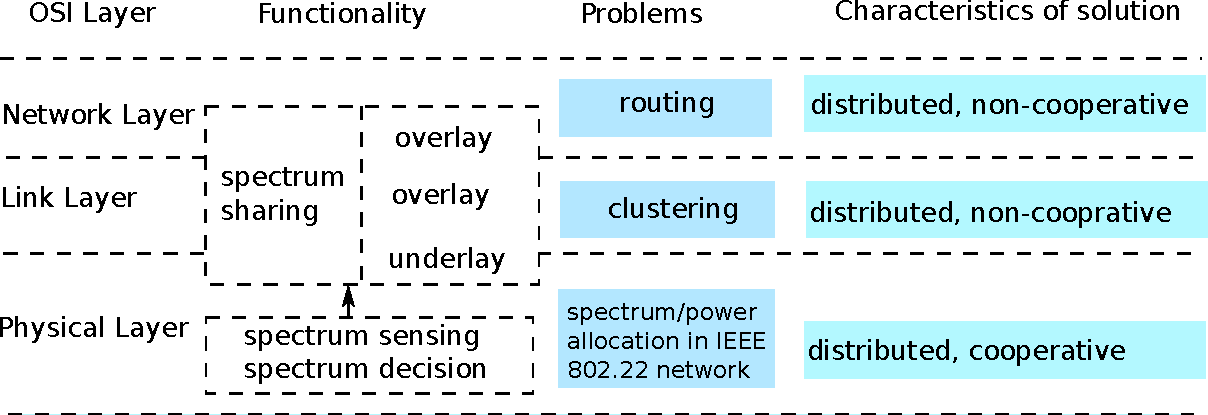
\includegraphics[width=\linewidth]{problemLocation.pdf}
  \caption{Spectrum management and the problems addressed in this thesis}
\label{problemLocation}
\end{figure}

%We focus on the distributed solutions for several correlated fundamental problems in CRN.
The interaction among autonomous secondary users is a common scene in CRN as there usually lacks central controller.
The secondary users endeavour to maximize their performance by choosing the channel and power, and meanwhile the accumulative interference caused on primary users should be below a threshold.
How to refrain the accumulative interference to exceed the threshold is a critical question, and whether the distributed decision made by each secondary user on channel and transmission power improves performance is worth considering.
After building the connected network with the chosen channel and transmission power, forming clusters with neighbours is a natural method to gain benefits, \ie more accurate spectrum sensing, from local cooperation.
How to form such clusters which can survive in front of the unpredictable activity of primary users is challenging.
Having had solid CRN infrastructure, it is time to deliver services via routing.
A light weight routing tailored for CRN is needed.
In the following, we give full problem statements for the mentioned challenges.



\subsection{Channel and Power Allocation in IEEE 802.22 Network}
%\subsubsection*{Utilize TV White Space}

As introduced in Section~\ref{ieee80222}, the TV white spectrum has appealing characteristics for secondary users, for instance, the TV spectrum spans wide frequency range, it is not used by TV services frequently and the spectrum availability lasts relatively longer.
There have been regulations, standards proposed to utilize TV spectrum, all of which rely on the centralized database to manage the spectrum usage, \ie channel and transmission power.

The conservative measures on the transmission power greatly restrict the full utilization of TV spectrum, and the channel allocation is not given consideration.
As to the former problem, based on the information of geographic locations and attenuation parameters, the upper bound of transmission could be relaxed, and the centralised database is a suitable place to conduct this work.
The later problem, at the first glance, has many similarities with the channel assignment problem which has been discussed extensively in the past decades, but the problem is unique as the transmission power on each user is different.
As a result, the interference caused between co-channel transmitters is not symmetric, which disables the solutions proposed for the channel assignment problems in conventional networks, \eg ad hoc networks, or mesh networks.




%This is very applicable as TV spectrum usage changes slowly, and the spectrum usage by TV stations is scheduled.
%the geographic location approach together with central database becomes more appealing in TW White Space (TVWS) utilization scenario. 
% FCC regulates portable secondary users to operate from channel 21 (512 MHz) to 51 (698 MHz), with the exception of channel 37. As to fixed secondary usage, the allowed spectrum band is from TV channel 2 (54 MHz) to TV channel 51, with TV channels 3, 4 and 37 being prohibited. Thus, the available TV spectrum is about 600 MHz wide. Compared to conventional unlicensed ISM bands in the 2.4 GHz and 5 GHz band, all together TVWS has more to offer.


\subsection{Robust Clustering in Ad Hoc Cognitive Radio Network}
Clustering is an important paving stone for the practical utilization of the unused portions of the licensed spectrum.
Clustering secondary users based on geographical proximity and other relevant properties together produces following benefits.
Firstly, it is more efficient to solve common control channel (\gls{CCC}) problem with cluster structure.
Dedicated CCC which is allocated to all nodes for the purpose of control information exchange is regarded to be under utilization.
Whereas, cluster based approaches group CR nodes into clusters based on their similarity of available unlicensed channels, so that the common channels within each cluster are used to carry the control messages~\cite{Lazos09}.
%whereas communication rendezvous, \ie the process to establish control channel between two CR users before they can communicate is proposed to be a economic solution.
%Within one cluster which is composed with CR nodes with similar available unlicensed channels, communication rendezvous can be accomplished within in shorter time~\cite{CommunicationRendezvous_ToN13}.
Secondly, cluster structure facilitates cooperative sensing and increases the sensing reliability~\cite{Sun07_clustering_spectrum_secsing}.
Thirdly, cluster structure supports coordinated channel switching and simplifies routing in ad-hoc cognitive radio networks~\cite{cluster_routing_2013ICC}.

The problem is defined by the following two metrics.
\begin{enumerate}
\item Abundance of control channels within cluster should be achieved.
A large number of control channels within cluster means high robustness.
When the current control channel gets occupied by primary user, cluster members can migrate to a new one and the cluster is maintained.
Besides, more control channels makes multiple concurrent transmission within cluster possible.
In this thesis, a distributed clustering algorithm which is especially designed to support robustness under active primary users is proposed.
Related works~\cite{Zhao07,Affinity_clustering_09icccn,Consensus_based_clustering12,clustering_globecom11} fail to pay attention to this aspect.

\item New scheme should be light weighted so that re-clustering can be quickly conducted when previous cluster is destroyed by primary user's activity.
When all the common channels are occupied by primary users, cluster head selection and following procedure is conducted by the cluster members autonomously.
\cite{LIU_TMC11_2} targets large number of control channels within cluster, but it intriguers high complexity.


%\item Efficient channel allocation scheme within and among clusters is needed, so that communication rendezvous between two clusters is quick. 
%Communication rendezvous means the process to establish control channel between two clusters before they can communicate .
%\cite{LIU_TMC11_2} proposes channel allocation in round robin manner, but it causes long time on communication rendezvous.
%\end{itemize}
%
%These requirements will be fulfilled by the scheme proposed in this thesis.
\end{enumerate}

\subsection{Geographic Routing in CRN with Spectrum Aware Virtual Coordinate}

Recent measurement in~\cite{measurement_Palaios14} shows the spectrum occupancy doesn't have significant spatial correlations between different locations.
It follows that licensed spectrum is used by primary users heavily in some areas, whereas in the other areas licensed spectrum is available over longer timespan for secondary users to use.
It is obvious to see that a routing path is better to go through the areas where primary users occupation is lower, as this alleviates or avoids the burden to cope with the changing or totally occupied spectrum when forwarding packets potentially with latency requirements.
Geographic routing is a natural choice to realize this geography sensitive routing path.
Geographic routing is light weight regarding the determination of next hop, and achieves high scalability in various wireless networks~\cite{geoRouing-qos-2009}. %
Merely knowing the geographic locations of its neighbours and the destination, a node is able to locally choose the next hop which has the smallest distance to the destination.
%As a result, control messages for route discovery are not necessary, and since the routing state maintained per node is independent on the network size, geographic routing scales perfectly.
However, in CRN dynamic link state renders geographic routing unsuccessful since packets are forwarded to the destination along the shortest path rather than avoiding areas heavily influenced by primary users.
%Coordinates indicate not only the physical distance among SUs, but also the transmission opportunities in between could leverage the strengths of geographic routing even in CRNs.
considering the available spectrum is geographically heterogeneous, applying geographic routing alike routing schemes in CRAHN is appealing, but the supporting coordinate system is missing.





\subsection{Research Questions}
Based on he previous analysis on the current secondary spectrum exploit, we conclude the problems into three distinct research questions.
In the remainder of this thesis, we will provide answers to these questions.

\textbf{Question Q1 - How to make full use of the TV spectrum, using the widely adopted network structure, preventing interference above threshold on primary TV receivers, and improve the performance of the secondary users.}

\textbf{Question Q2 - How to make the secondary users to form robust clusters against primary users' unpredictable activity?}

\textbf{Question Q3 - How to make use of the statistic information of the spectrum availability, so as to realize light weight geographic routing in CRN.}




\section{Contributions}
Because of the characteristics of the problems, distributed schemes are adopted, and in order to coordinate the interaction between secondary users, game theory is used to formulate the problem and derive algorithms.
We illustrate the contribution of this thesis by addressing the aforementioned questions.


\subsection*{Contribution 1: Distributed Channel and Power Allocation in IEEE 802.22 Network}



In this thesis we cope with a special channel allocation problem where symmetric interaction doesn't exist, \ie transmission power is identical among CR users, or the propagation path loss is not symmetric. 
The asymmetry disables the heuristic distributed schemes provided in~\cite{Ko_DistributedCA}, and makes channel allocation problem not to fit into the congestion game model proposed in~\cite{allerton08_liu} which is the first paper to discuss channel allocation from the respective of game theory.
We innovatively formulate this problem in to a canonical congestion game by utilizing the centralized database in TV white space scenario, and derive efficient distributed channel selection strategy.
%and apply it on different cognitive radio networks.
%rethink channel allocation problem from the perspective of game theory, particularly,


This thesis addresses following two problems,
\begin{itemize}
\item Decide the maximal downlink transmission power.
Both FCC regulation and 802.22 standard try to make TVBD transparent to incumbent users, but as long as TV system is not affected, i.e. certain quality of service is fulfilled, the strict restriction on unlicensed users can be relaxed so that more TVWS can be provided~\cite{multipleIntf_pimrc11}. 
Abiding by the operation paradigm using data base, we investigate the maximal downlink transmission power for TVBDs by solving optimization problem where the cumulative interference on TV receivers is under a threshold.

\item Distributed spectrum allocation scheme for TVBDs.
According to 802.22 regulation, spectrum allocation is done centrally in TV database, this is not realistic when TVBDs belong to different economic interest groups, thus a distributed solution is needed.
We propose efficient distributed scheme to allocate the TV channels in order to improve the quality of service of TVBDs.
The major difference between our scheme and other spectrum allocation lies in that the downlink transmission power on different channel is different.
We formulate this problem into a canonical congestion game, and derive the distributed algorithm from the best response behaviour of the player in the game. 
\end{itemize}





\subsection*{Contribution 2: Light Weight Robust Clustering in CRAHN}
We propose a decentralized clustering approach, which is able to form clusters whose sizes are not far away from the desired size, and the generated clusters are more robust than other robust clustering scheme, \ie more secondary users residing in clusters against increasing affection from primary users.
Compared to previous work, our proposed scheme involves much less control messages, and the generated clusters are significantly more robust.
We formulate one procedure of the scheme into a singleton congestion game, which permits Nash equilibrium when CR users adopt  best response strategy. 
%building more homogeneous clusters with respect to their size and forcing nodes with a high connectivity degree to the border of a cluster (making the cluster therefore more robust regarding connectivity loss to its neighbor).
%For our scheme we can prove convergence in cluster formation phase and resolve ambiguities with respect to cluster membership in a game-theoretic setting. 
On the basis of proposed scheme, we propose a light weighted version of ROSS, which requires exchanging less overheads.
%We leave the channel selection undiscussed.







\subsection*{Contribution 3: Spectrum Aware Virtual Coordinates in CRN}


In this paper we propose SAViC, spectrum aware virtual coordinates for secondary users in multi-channel multi-hop CRN where secondary users are source limited.
Virtual coordinate is independent of real geographic position, but decided by certain properties of the media among nodes, for instance, link quality or hop numbers~\cite{gpsfree05infocom}.
The proposed virtual coordinate depicts the availability of licensed spectrum influenced by primary users, on top of which geographic routing decides the next hop with Euclidean distance metric, and unconsciously detours the primary affecting area, or cuts through the area with better access opportunity.
This routing paradigm imposes little computation and communication cost on secondary users after assigning virtual coordinate, besides, it doesn't need real geographic location which is employed in ~\cite{search_geo_routing_chowdhury, routing-crn-jsac12}.

This scheme is composed with two steps,
\begin{itemize}
\item Design virtual coordinates so that virtual coordinates of any two secondary users reflect both geographic distance and opportunistic spectrum availability between them.
We design them based on statistics of primary user’s ON/OFF states which are obtained from local spectrum sensing.

\item After deciding on the next hop, we adopt a lightweight heuristic method to decide which channel to transmit packet when multiple licensed channels exist in the network.


\end{itemize}

To summarize, as the Euclidean distance between two secondary users based on spectrum aware virtual coordinate reflects the availability of unlicensed channel in between from the angel of historical statistics, virtual coordinate contributes a large part to deciding on the on the next hop. 











\section{Outline}
The structure of this thesis is as follows.
In chapter 2, we introduce the tools used in solving the problems, \ie game theory and optimization. 
Chapter 3 introduces the work on utilization of TV white space.
The robust clustering problem is addressed in Chapter 4.
In Chapter 5, virtual coordinate based on geographic routing is designed and geographic routing runs on the top of it.
Finally, Chapter 7 concludes the thesis by summarizing our contributions and discussing the future work.




